\documentclass[final]{fhnwreport}         %[mode] = draft or final
%%---Main Packages-----------------------------------------------------------------------
\usepackage[english, ngerman]{babel}	%Mul­tilin­gual sup­port for LaTeX
\usepackage[T1]{fontenc}				      %Stan­dard pack­age for se­lect­ing font en­cod­ings
\usepackage[utf8]{inputenc}				  %Ac­cept dif­fer­ent in­put en­cod­ings
\usepackage{lmodern}                 %The newer Font-Set
\usepackage{textcomp}					      %LaTeX sup­port for the Text Com­pan­ion fonts
\usepackage{graphicx} 					      %En­hanced sup­port for graph­ics
\usepackage{float}						        %Im­proved in­ter­face for float­ing ob­jects
%\usepackage{ifdraft}                %Let you check if the doc is in draft mode

%%---Useful Packages---------------------------------------------------------------------
\usepackage[pdftex,dvipsnames]{xcolor}  %Driver-in­de­pen­dent color ex­ten­sions for LaTeX
\usepackage{csquotes}                   %Simpler quoting with \enquote{}
\usepackage{siunitx} 					     %A com­pre­hen­sive (SI) units pack­age
\usepackage{listings}					     %Type­set source code list­ings us­ing LaTeX
\usepackage[bottom]{footmisc}			  %A range of foot­note op­tions
\usepackage{footnote}					     %Im­prove on LaTeX's foot­note han­dling
\usepackage{verbatim}					     %Reim­ple­men­ta­tion of and ex­ten­sions to LaTeX ver­ba­tim
\usepackage[textsize=footnotesize]{todonotes} %Mark­ing things to do in a LaTeX doc­u­ment
\usepackage{lipsum}              % Gives you access to blindtext

%%---Tikz Packages-----------------------------------------------------------------------
%\usepackage{standalone}
%\usepackage{tikz}
%\usepackage{circuitikz}
%\usetikzlibrary{arrows}
%\usetikzlibrary{calc}
%\usetikzlibrary{intersections}

%%---Math Packages-----------------------------------------------------------------------
\usepackage{amsmath}					    %AMS math­e­mat­i­cal fa­cil­i­ties for LaTeX
%\usepackage{amssymb}					  %Type­set­ting symbols (AMS style)
%\usepackage{array}						  %Ex­tend­ing the ar­ray and tab­u­lar en­vi­ron­ments
%\usepackage{amsthm}					    %Type­set­ting the­o­rems (AMS style)

%%---Table Packages----------------------------------------------------------------------
\usepackage{tabularx}					  %Tab­u­lars with ad­justable-width columns
%\usepackage{longtable}
\usepackage{multirow}					  %Create tab­u­lar cells span­ning mul­ti­ple rows
\usepackage{multicol}					  %In­ter­mix sin­gle and mul­ti­ple columns

%%---PDF / Figure Packages---------------------------------------------------------------
\usepackage{pdfpages}					  %In­clude PDF doc­u­ments in LaTeX
\usepackage{pdflscape}					  %Make land­scape pages dis­play as land­scape
%\usepackage{subfig}					    %Fig­ures di­vided into sub­fig­ures

%%---Other Packages----------------------------------------------------------------------
%\usepackage{xargs}              %De­fine com­mands with many op­tional ar­gu­ments


%%---Main Settings-----------------------------------------------------------------------
\graphicspath{{./graphics/}}			%Defines the graphicspath
%\geometry{twoside=false}				%twoside=false disables the "bookstyle"
\setlength{\marginparwidth}{2cm}
\overfullrule=5em						    %Creates a black rule if text goes over the margins => debugging

%%---User Definitions--------------------------------------------------------------------
%%Tabel-Definitions: (requires \usepackage{tabularx})
\newcolumntype{L}[1]{>{\raggedright\arraybackslash}p{#1}}    %column-width and alignment
\newcolumntype{C}[1]{>{\centering\arraybackslash}p{#1}}
\newcolumntype{R}[1]{>{\raggedleft\arraybackslash}p{#1}}					            %loads all packages, definitions and settings

%%%%% Logo: Hocvhschule HTU oder HSI, Sprache DE oder EN:
%\newcommand{\logofilename}{FHNW_HTU_EN}
\newcommand{\logofilename}{FHNW_HSI_DE}
%\newcommand{\logofilename}{FHNW_HSI_EN}
%%%%%
%%%%% Bibliographie entweder im IEEE- oder im APA-Stil:
\usepackage[style=ieee,urldate=comp,backend=biber]{biblatex}
%\usepackage[style=apa,urldate=comp,backend=biber]{biblatex}
%%%%%
\usepackage{xcolor}

\usepackage[automake]{glossaries}

\newglossaryentry{IoT}{
    name={IoT},
    description={Internet of Things, Vernetzung physischer Geräte}
}

\makeglossaries



\lstdefinestyle{customtypescript}{
  belowcaptionskip=1\baselineskip,
  breaklines=true,
  frame=single,
  xleftmargin=\parindent,
  numbers=left,
  language=Java, % absichtlich Java für bessere Farben
  showstringspaces=false,
  basicstyle=\footnotesize\ttfamily,
  keywordstyle=\color{black}, % Verhindert falsches Blau bei z. B. „label“
  commentstyle=\itshape\color{green!60!black},
  identifierstyle=\color{black},
  stringstyle=\color{orange!80!black},
  numberstyle=\tiny\color{gray!70},
  rulecolor=\color{gray!70},
  backgroundcolor=\color{gray!5},
  morekeywords={}, % verhindert zusätzliche Keywords
  literate={ß}{{\ss}}1
           {Ö}{{\"O}}1 {Ä}{{\"A}}1 {Ü}{{\"U}}1
           {ü}{{\"u}}1 {ä}{{\"a}}1 {ö}{{\"o}}1
           {`}{\textasciigrave}1
           {'}{{\textquotesingle}}1
           {"}{{\textquotedbl}}1
}


\addbibresource{literature/beispiel_bib.bib}
											
\title{Code Assist und Navigation für IoT-Konfigurationen
	mit Language Server Protocol}  %Project Title
\author{Bachelor Thesis}    %Document Type => Technical Report, ...
\date{Windisch, August 2025}               %Place and Date

\begin{document}

\pagenumbering{roman}	

%%---TITLEPAGE---------------------------------------------------------------------------
\selectlanguage{ngerman}                  %ngerman or english
\maketitle

\vfill

\begin{figure}[H]
\centering
%\includegraphics[width=\linewidth]{} % Pic Title
\end{figure}

\vfill

\begin{tabular}{@{}p{5cm} l}
Student          			&    Gianni Parrillo\\[2ex]        
Experte						&    Raphael Schweizer Iuliano\\[2ex]
Fachbetreuer				&    Prof. Dr. Dominik Gruntz\\
							&	 Daniel Kröni\\[2ex]
Auftraggeber				&    Fabrizio Parrillo, Colomba Link GmbH\\[3ex]
Projektnummer				&    $25FS\_IMVS39$\\[4ex]
\multicolumn{2}{@{}l}{Fachhochschule Nordwestschweiz, Hochschule für Informatik}
\end{tabular}

\vspace*{4ex}
% Beispiel für Logo Industriepartner
\begin{tikzpicture}[remember picture,overlay,every node/.style={anchor=north east}]
  \node at (current page.north east) [xshift=-1cm, yshift=-0.5cm] {
\includegraphics[width=4cm]{colomba.png}};
  % Photo by Stoica Ionela on Unsplash
\end{tikzpicture}

\clearpage


%%---ABSTRACT----------------------------------------------------------------------------
\selectlanguage{ngerman}				%ngerman or english
\thispagestyle{empty}
\section*{Abstract}
Die Colomba ....

\vspace{2ex}

\textbf{Keywords:}

tic, tac tooo

\clearpage

%\section*{Vorwort / Dank}




%%---TABLE OF CONTENTS-------------------------------------------------------------------	
\selectlanguage{ngerman}				%ngerman or english
\tableofcontents
\clearpage
\listoffigures
\newpage
\addcontentsline{toc}{section}{Listingverzeichnis}
\renewcommand{\lstlistlistingname}{Listingverzeichnis}
\lstlistoflistings
\newpage
\addcontentsline{toc}{section}{Glossar}
\printglossaries

\newpage
%%---TEXT--------------------------------------------------------------------------------
\pagenumbering{arabic}

\section{Einleitung}

\subsection{Ausgangslage und Problemstellung}
Die modulare Entwicklung von Software wird im Bereich der IoT-Systeme zunehmend relevant. Mit der steigenden Anzahl vernetzter Geräte und wachsenden Datenmengen nimmt die Komplexität zu. Modulare Lösungen gelten als zentraler Bestandteil aktueller IoT Ansätze \cite{IoT}.

Die Colomba Link GmbH betreibt mit Monidas eine IoT-Plattform für industrielle Anwendungen. Sie verwaltet Daten wie Organisationen, Projekte, Benutzer, Sensoren sowie zugehörige Überwachungs- und Benachrichtigungsregeln. Mit zunehmender Anzahl an Sensoren, Regeln und Benachrichtigungen steigt der Aufwand für technische Mitarbeitende. Sie konfigurieren die Sensoren gemeinsam mit dem Kunden und installieren diese Vorort. Die Konfiguration erfolgt über die Webplattform. Sensoren, Regeln und Benachrichtigungen werden einzeln erstellt und über mehrere Eingabemasken miteinander verknüpft.

Um diesen Prozess zu optimieren, wurde im Rahmen eines Vorprojekts ein Proof of Concept erstellt. Ziel war es, die Machbarkeit einer alternativen Schnittstelle in Form einer VS Code Extension zu evaluieren. Dafür wurde ein Prototyp entwickelt, der das Domänenmodell in einer TreeView darstellt und die Bearbeitung über den JSON-Editor ermöglicht.
 
Im Proof of Concept war das Domänenmodell hardcodiert. Jede Änderung am Datenmodell erforderte eine Anpassung im Quellcode. Die Validierung und Autovervollständigung im Editor wurden über statische JSON-Schemas realisiert, die vom Standard-JSON-Language-Server verarbeitet wurden. Für weiterführende Funktionen wie Jump to Definition ist ein eigener Language Server erforderlich.


\subsection{Zielsetzung}

Ziel dieser Bachelorarbeit ist die Analyse und Umsetzung einer modularen Lösung, welches ein Datenmodell als virtuelles Filesystem darstellt. Die Lösung soll mit verschiedenen Datenstrukturen funktionieren. Bei Änderungen und der Erstellung des Datenmodells ist keine Anpassung des Codes notwendig. Es wird untersucht, wie sich komplexe Strukturen wie in IoT-Systemen damit abbilden lassen. Darauf aufbauend wird ein eigener Language Server entwickelt, der die Bearbeitung der Daten im Editor unterstützt. Er stellt Funktionen wie Autovervollständigung, Validierung und Navigation bereit. 

Angesichts der im vorherigen Kapitel beschriebenen Problematik ergeben sich die folgenden Leitfragen, welche im Mittelpunkt dieser Arbeit stehen:

\begin{itemize}

\item Wie kann ein virtuelles Filesystem in VS Code so umgesetzt werden, dass es sich allein durch ein  Datenmodell steuern lässt und auch komplexe Strukturen unterstützt?

\item Wie kann ein eigener Language Server so entwickelt werden, dass er strukturierte Datenmodelle im Editor unterstützt und Funktionen wie Autovervollständigung, Validierung und Navigation bereitstellt?
\end{itemize}

Zur Beantwortung dieser Fragen werden Architektur, Umsetzung und Integration der Komponenten analysiert und praktisch umgesetzt.

\subsection{Abgrenzung}
Im Rahmen dieser Arbeit werden folgende Themenbereiche nicht behandelt. Die entwickelte Lösung wird nicht in das Produktivsystem von Monidas integriert. Es findet keine Anbindung an die bestehende Webplattform oder das Backend statt. Die Evaluation erfolgt ausschliesslich anhand des Datenmodells, ohne produktive Abläufe zu beeinflussen.

Nicht berücksichtigt werden ausserdem Funktionen zur gleichzeitigen Nutzung durch mehrere Benutzer, die Benutzerverwaltung, Authentifizierungsprozesse sowie die Rechtevergabe. Auch Themen wie Datensicherheit, Performanceoptimierung, Datenmigration oder die Anbindung externer Systeme sind nicht Bestandteil dieser Arbeit.


\subsection{Leserführung}

Die vorliegende Bachelorarbeit ist in sechs Themenkomplexe untergliedert. Kapitel 1 umfasst die Einführung in die Arbeit und beschreibt die Ausgangslage, Problemstellung, Zielsetzung sowie die Abgrenzung. Es wird erläutert, weshalb die Weiterentwicklung einer bestehenden VS Code Extension zur Bearbeitung von Konfigurationsdaten im Kontext der Monidas-IoT-Plattform untersucht wird.

Kapitel 2 beschreibt die eingesetzte Datenbank und ihren konkreten Einsatz im Projekt. Es wird aufgezeigt, welche Funktionen die Datenbank bereitstellt und welche zusätzlichen Regeln im Datenbankschema definiert wurden, um das Verhalten der Anwendung zu steuern. Ein Beispielmodell dient als Referenz für die gesamte Arbeit. Zudem wird erläutert, wie das Datenmodell zur Laufzeit analysiert und für das virtuelle Dateisystem und den Editor verfügbar gemacht wird.

\section{Monidas Plattform}

Info:
Geplant ist hier, ein vereinfachtes Domänenmodell der Monidas-Plattform zu beschreiben. Es ist derzeit noch offen, ob die eingesetzten Technologien bereits hier erläutert werden oder erst in den entsprechenden Kapiteln (VFS, LSP). Die Evaluation des Monidas-Domänenmodells sowie des daraus resultierenden Schemas erfolgt erst am Ende dieser Arbeit, nachdem sämtliche Komponenten vorgestellt wurden. Dabei werden notwendige Anpassungen im Schema identifiziert, um die entwickelte Lösung erfolgreich umzusetzen.
%\section{Datenmodell und Schema}
Leseeinführung 

\subsection{Struktur}
Aufbau der Typenstruktur, Felder, Referenzen.

\subsection{Constraints}

\begin{itemize}
	\item Definition von constraints wie notNull, existsIn
	\item Nutzung zur Validierung im VFS und zur Vervollständigung im LSP
\end{itemize}

\subsection{Beispielmodell}
Einheitliches Modell für alle Kapitel

\subsection{Analyse des Schemas}
Traversieren des Schemas: - Erkennen von Wurzeln (Root-Typen) - Analyse von Referenzpfa 
den - Erkennung von moeglichen Zyklen


%\section{Architekturübersicht}
\label{kap:Architek}
Nach der Vorstellung der verwendeten Technologien beschreibt dieser Abschnitt den Aufbau der Gesamtarchitektur. Für das Lesen der Arbeit stellt die Übersicht eine Orientierungshilfe dar, um die technische Gliederung der Lösung von Beginn an nachvollziehbar zu machen. Die nachfolgende Beschreibung orientiert sich an der nummerierten Abbildung~\ref{fig:architekturuebersicht}, um das Zusammenspiel der Komponenten sowie den Datenfluss übersichtlich darzustellen und nachvollziehbar zu machen.

Die entwickelte Lösung ist in drei Hauptbereiche unterteilt: (1) Datenbank, (2) Backend und (3) VS Code Extension.

Die Graphdatenbank (1) speichert die Entitäten der Anwendung und liest beim Start das definierte Datenbankschema (1.1) ein, welches deren Struktur, Typen und mögliche Beziehungen festlegt.

Im Backend (2) übernehmen zwei Controller die Kommunikation mit der Datenbank. Der VFS Controller (2.1) verarbeitet Anfragen des virtuellen Filesystems. Der LSP Controller (2.2) liefert dem VFS Language Server (2.3) die Daten, welche dieser benötigt, um Anfragen des Editors für Validierung, Autocompletion und Go-to-Definition zu beantworten.

Innerhalb von Visual Studio Code (3) bestehen zwei Extensions mit getrennten Verantwortlichkeiten. Die Virtual Filesystem Extension (3.1) stellt eine Benutzeroberfläche im Explorer und im Editor bereit, über welche Datenobjekte navigiert sowie erstellt, geöffnet, bearbeitet und gespeichert werden können. Die VFS Language Client Extension (3.2) unterstützt den Editor mit Funktionen wie Validierung und Autovervollständigung. Die Aktivierung erfolgt beim Öffnen des Editors, wobei die Extension auf Aktionen wie das Bearbeiten von Dateien reagiert.

\begin{figure}[H]
    \centering
    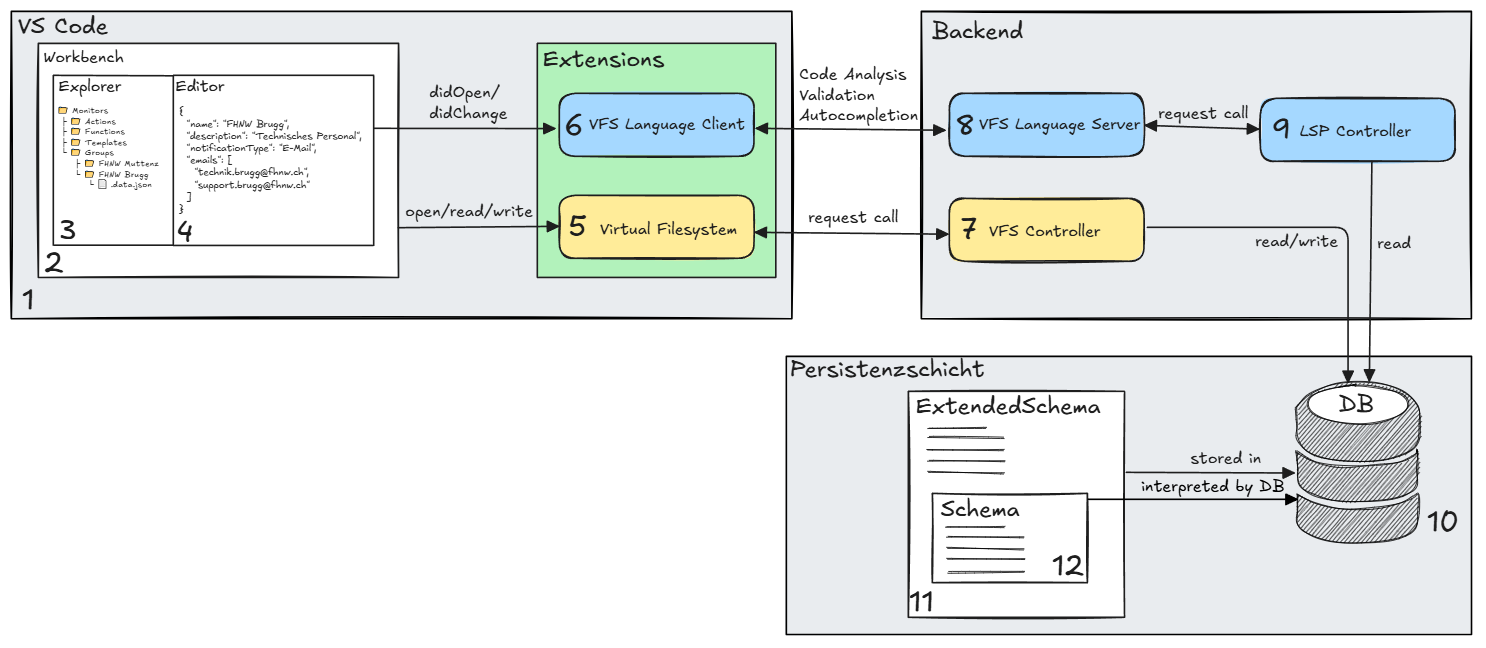
\includegraphics[width=1\linewidth]{arch.png}
    \caption{Architektur desMonidas Code Assist Navigator}
    \label{fig:architekturuebersicht}
\end{figure}

\section{Datenbankschema}
\label{kap:dbschema}
In diesem Kapitel werden die Anforderungen an das Datenbankschema beschrieben. Anschliessend wird ein vereinfachtes Domänenmodell vorgestellt, das als Grundlage für die weiteren Kapitel dient. Danach folgen die Beschreibung der Lösungsansätze und deren Umsetzung. Diese bildet die Grundlage für die Erläuterungen des Kapitel~\ref{kap:vfs} -~\ref{kap:lsp}.

\subsection{Anforderungen}
\label{abb:anforderungen}
Das Ziel dieser Bachelorarbeit ist die Entwicklung einer generischen, datenmodellgetriebenen Anwendung zur Verwaltung von IoT-Konfigurationen. Die Anwendungslogik soll dabei vollständig aus einem definierten Datenmodell abgeleitet werden, sodass Anpassungen im Quellcode vermieden werden. Daraus ergeben sich drei Anforderungen an das Datenbankschema: Erstens müssen Einstiegspunkte im Schema definiert werden, damit die Anwendung erkennt, wo der Verwaltungsprozess beginnt. Zweitens muss das Schema zusätzliche Validierungen unterstützen, da die verwendete Datenbanktechnologie Selva nur grundlegende Datentyp-Prüfungen bereitstellt. Drittens soll es möglich sein, zusätzliche Informationen wie beispielsweise Blattknoten oder potenzielle zyklische Verweise aus dem Schema abzuleiten, ohne dass diese im Schema definiert werden müssen.

\subsection{Domänenmodell}
\label{abb:domaenenmodell}
Das in Abschnitt~\ref{abb:tech} beschriebene Domänenmodell ist zu komplex, um es unverändert in der entwickelten Lösung zu verwenden. Deshalb wird zunächst ein vereinfachtes Modell definiert, das für die Umsetzung geeignet ist. Die Übertragbarkeit auf das Domänenmodell der Monidas-Plattform wird in Kapitel~\ref{kap:eva} untersucht.

Das für diese Arbeit verwendete Domänenmodell ist in Abbildung~\ref{ab:con} dargestellt und bildet ein typisches Szenario aus dem E-Commerce-Bereich ab. Das Modell besteht aus den fünf Entitäten: \textit{Customer}, \textit{Address}, \textit{Order}, \textit{LineItem} und \textit{Product}. Ein \textit{Customer} (Kunde) verfügt über Angaben wie Vorname, Nachname und eine E-Mail-Adresse. Jeder Kunde besitzt mehrere Adressen (\textit{Address}) und kann mehrere Bestellungen (\textit{Order}) tätigen. Eine Adresse umfasst die Strasse, Stadt sowie das Land und gehört eindeutig zu einem Kunden. Jede Bestellung besitzt eine Rechnungsadresse (\textit{billingAddress}) und optional eine Lieferadresse (\textit{shippingAddress}). Eine Bestellung besteht aus mindestens einer Bestellposition (\textit{LineItem}), welche jeweils ein Produkt (\textit{Product}) mit einer definierten Menge und einem Einzelpreis referenziert. Ein Produkt enthält eine eindeutige Beschreibung sowie einen Preis.

\begin{figure}[H]
    \centering
    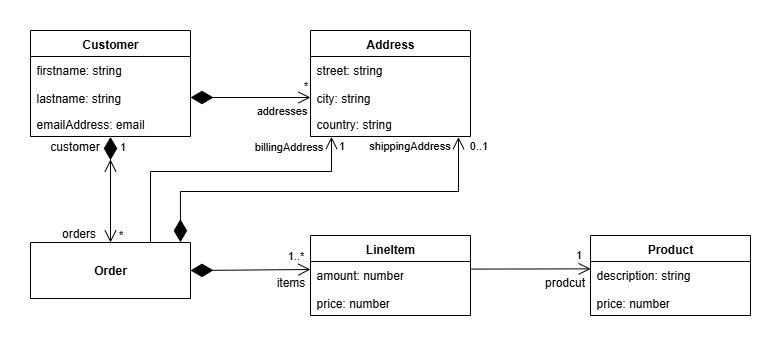
\includegraphics[width=0.8\linewidth]{Bsp_UML.png}
    \caption{Vereinfachtes Domänenmodell im E-Commerce-Kontext}
    \label{fig:uml_domaenenmodell}
\end{figure}

\subsection{Schemaerweiterungen}
Um die Anforderungen der Anwendung erfüllen zu können, mussten Erweiterungen am bestehenden Schema vorgenommen werden. Diese umfassen die Definition von Einstiegspunkten (Roots), Bedingungen (Constraints) sowie die dynamische Ableitung zusätzlicher Informationen.

\label{ab:con}
\subsubsection{Roots}
Unter dem Begriff «Roots» werden die im Schema definierten Einstiegspunkte verstanden. Diese bestimmen, bei welchen Entitäten die Navigation im virtuellen Filesystem beginnt. Für jeden Root wird ein Label festgelegt, das im Filesystem als Ordnername angezeigt wird. Dieses Label wird direkt im Schema definiert und kann unabhängig vom Namen der Entität frei gewählt werden.

Im E-Commerce-Domänenmodell (siehe Abbildung \ref{fig:uml_domaenenmodell}) könnten beispielsweise die Entitäten \textit{Customer} mit dem Label \textit{Customers} und \textit{Product} mit dem Label \textit{Products} als Roots definiert werden.

\subsubsection{Constraints}
Unter «Constraints» werden in dieser Thesis Bedingungen verstanden, die das Standardverhalten der Applikation gezielt ergänzen oder einschränken. Sie stellen sicher, dass die Daten bestimmte Anforderungen erfüllen und inhaltlich konsistent bleiben. Diese Bedingungen werden ausschliesslich von der Anwendungslogik geprüft und nicht von der Datenbank selbst.

Das Standardverhalten der Applikation sieht vor, dass neue Objekte direkt innerhalb ihres übergeordneten Knotens erstellt werden. Dieses Verhalten folgt einer Parent-Child-Hierarchie. Das Referenzieren eines bereits bestehenden Objekts ist standardmässig deaktiviert. Mit „Referenzieren“ wird in dieser Arbeit verstanden, dass beispielsweise bei einer Bestellung keine neue Adresse erstellt, sondern eine bereits existierende Adresse zugeordnet wird.

Werden jedoch zusätzliche Bedingungen benötigt, um das Standardverhalten gezielt zu erweitern, stehen die folgenden Constraints zur Verfügung: Pflichtfeld (notNull), bidirektionale Verknüpfung (bidirektional), Verbot der Erstellung neuer Objekte (denyCreation) und Erlaubnis zum Referenzieren bestehender Objekte (allowReference). Zur Veranschaulichung dieser Constraints dient folgendes Beispiel aus dem E-Commerce-Domänenmodell:

Beim Erstellen eines neuen Kunden ist die Angabe einer E-Mail-Adresse zwingend erforderlich (notNull), andernfalls ist das Speichern nicht möglich. Anschliessend erstellt der Kunde zwei Adressen, beispielsweise eine Heimadresse und eine Arbeitsadresse, welche eindeutig diesem Kunden zugeordnet sind. Möchte der Kunde eine Bestellung tätigen, ist dafür zwingend die Angabe einer Rechnungsadresse (billingAddress) erforderlich (notNull). Innerhalb der Bestellung ist das Erstellen einer neuen Rechnungsadresse technisch nicht möglich, da dies explizit deaktiviert wurde (denyCreation). Stattdessen muss eine bereits vorhandene Adresse ausgewählt werden (allowReference), beispielsweise die zuvor erstellte Arbeitsadresse. Darüber hinaus muss jede Bestellung mindestens eine Bestellposition enthalten (notNull). Diese Bestellposition wird direkt im Kontext der Bestellung erstellt und muss zwingend auf ein bereits bestehendes Produkt (Product) verweisen (allowReference, denyCreation). Optional kann zudem eine Lieferadresse angegeben werden. Diese Lieferadresse wird direkt im Kontext der Bestellung erstellt und existiert ausschliesslich dort. Das Referenzieren bereits bestehender Adressen, beispielsweise der Heim- oder Arbeitsadresse, ist hierbei technisch deaktiviert und daher nicht möglich (Standardverhalten).

\subsubsection{Schema Analyse}
\label{sec:dynamischerAb}
Die zuvor beschriebenen Schemaerweiterungen wie Constraints und Roots werden statisch definiert. Eine weitere Information, nämlich ob ein Referenzfeld zu einem Blattknoten (\textit{isLeaf}) führt, lässt sich hingegen durch eine Schema-Analyse ableiten. Ein Blattknoten bezeichnet hierbei einen Knoten, dessen Entitätstyp keine weiteren ausgehenden Referenzen besitzt. Diese ermittelte Information wird genutzt, um Darstellungs- und Bearbeitungslogiken innerhalb des virtuellen Filesystems zu steuern. Die konkrete Verwendung wird detailliert in Kapitel~\ref{kap:vfs} erläutert. Dies wird direkt im Schema ergänzt, wodurch sich der Modellierungsaufwand reduziert und die Flexibilität für Erweiterungen steigt.

Für die Schema-Analyse wird das Schema als gerichteter Graph interpretiert. Entitätstypen wie \textit{Customer}, \textit{Order}, \textit{Address}, \textit{LineItem} und \textit{Product} bilden dabei die Knoten, während Referenzfelder wie \textit{addresses}, \textit{billingAddress}, \textit{shippingAddress}, \textit{customer}, \textit{items} und \textit{product} die gerichteten Kanten darstellen. Zur Traversierung des Graphen wird der Algorithmus der Tiefensuche (Depth-First Search, DFS) verwendet. Dabei handelt es sich um einen Graphen-Algorithmus, der von einem Startknoten ausgehend zunächst einen Pfad vollständig verfolgt, bevor zurückgegangen und der nächste Pfad untersucht wird. 

\begin{figure}[H]
    \centering
    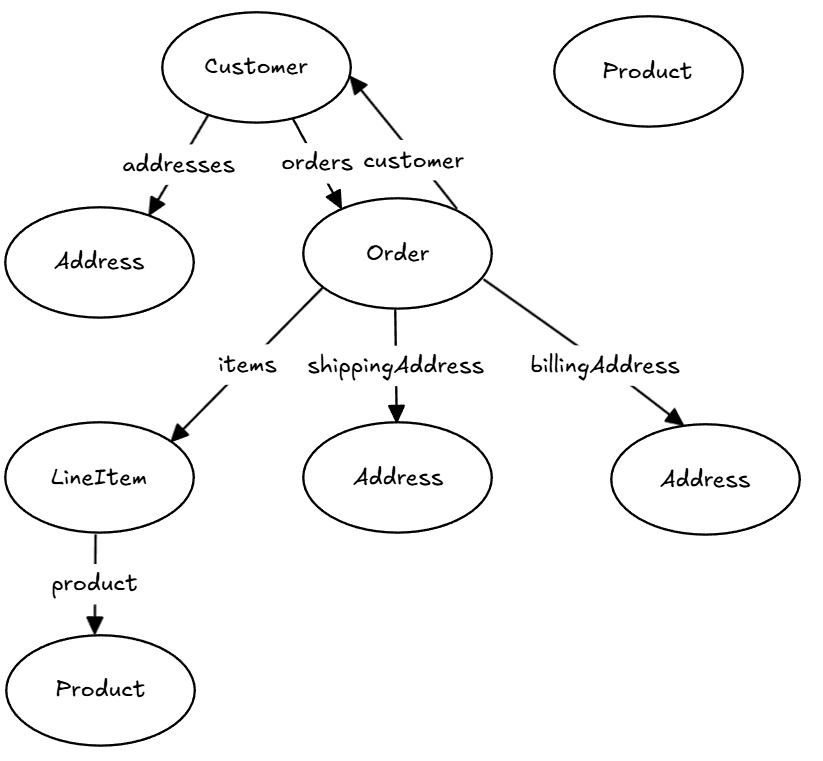
\includegraphics[width=0.8\linewidth]{dag.png}
    \caption{Gerichtete Graphdarstellung des E-Commerce-Datenbankschemas}
    \label{fig:dag}
\end{figure}
\newpage

Im Rahmen der Lösungsfindung wurden weitere Ansätze zur Informationsableitung geprüft. Einer dieser Ansätze bestand darin, sämtliche möglichen URIs bereits im Vorfeld aus dem Schema abzuleiten. Ein URI (Uniform Resource Identifier) bezeichnet hierbei einen eindeutigen Pfad, der sich aus der Abfolge von Referenzfeldern (gerichteten Kanten) und Instanzen von Entitätstypen (Knoten) zusammensetzt. Eine Instanz bezeichnet dabei ein konkretes Datenobjekt, das auf Basis einer im Schema definierten Entität erzeugt wurde. Beispielsweise ergibt sich ein URI aus einer Abfolge wie:

\begin{center}
\texttt{Customers/\{customerId\}/Orders/\{orderId\}}
\end{center}

Ziel dieses Ansatzes war es, alle gültigen URI-Muster im Vorfeld zu ermitteln, um URIs zur Laufzeit validieren zu können. Dieses Vorgehen ist allerdings nur geeignet, wenn im Schema keine Zyklen auftreten. Sobald zyklische Referenzen vorhanden sind, entstehen theoretisch unendlich viele URI-Kombinationen. Daher lässt sich dieser Ansatz bei zyklischen Schemata nicht allgemein anwenden.

Ein weiterer untersuchter Ansatz bestand darin, die genaue Pfadtiefe eines URI bereits im Voraus zu ermitteln. Da jedoch eine vollständige Abbildung aller möglichen URIs vorab nicht realisierbar war und sich die Pfadtiefe ohnehin einfach direkt aus dem URI während einer Anfrage ableiten lässt, erwies sich dieser Ansatz letztlich als nicht zielführend und wurde verworfen.
%hasPossbileCycle
%\subsection{Bereitstellung und Zugriff}

\subsection{Umsetzung}

\subsubsection{Roots und Constraints}
Die Definition von Einstiegspunkten („Roots“) sowie zusätzlichen Validierungen („Constraints“) erfordert eine Erweiterung der ursprünglichen TypeScript-Typdefinition aus der Colombalink-Bibliothek. Für die Umsetzung wurde das bestehende Schema aus der Colombalink-Bibliothek angepasst. Dabei wurde die Typdefintion Schema erweitert, um die Definition von Roots und Constraints zu ermöglichen. Die dafür notwendigen TypeScript-Features wie Omit, Intersection Types, Union Types und Generics stellten sicher, dass diese Erweiterung umgesetzt werden konnte~\cite{typescript:handbook}. Das Ergebnis ist ein erweitertes Schema, das den Anforderungen aus Abschnitt~\ref{abb:anforderungen} entspricht. Die genaue technische Umsetzung befindet sich im Anhang in Listing~\ref{lst:extended-schema}.

Im vorherigen Abschnitt wurde bereits erläutert, wie im konkreten E-Commerce-Domänen\-modell die Entitäten \textit{Customer} und \textit{Product} als Roots definiert wurden, sowie welche Constraints für die Entität \textit{Order} gesetzt wurden. Im nachfolgenden Listing~\ref{lst:con} ist dargestellt, wie dies im erweiterten Schema definiert werden können.

\newpage
\lstinputlisting[
caption={Definition von Roots und Constraints im erweiterten Schema},
label={lst:con},
style=customtypescript
]{listings/con.json}

\newpage
\subsubsection{Schema Analyse}
Die technische Umsetzung der Schema-Analyse erfolgt mithilfe einer rekursiven Tiefensuche. Ausgangspunkte der Traversierung sind die zuvor definierten Einstiegspunkte (\textit{Customer} und \textit{Product}, siehe Abschnitt~\ref{ab:con}).

Während der Tiefensuche wird jeder besuchte Entitätstyp (Knoten) erfasst. Wird ein bereits besuchter Knoten erneut erreicht, deutet dies auf einen möglichen Zyklus hin und die weitere Traversierung entlang dieses Pfades wird beendet. Hat ein referenzierter Knoten keine weiteren ausgehenden Referenzen, wird das Feld \texttt{isLeaf} gesetzt, um ihn als Blattknoten zu kennzeichnen.

Das Ergebnis der Schema-Analyse für das E-Commerce-Schema ist in Tabelle~\ref{tab:schema-analyse-dfs} dargestellt. Der zugehörige Code befindet sich im Anhang (Listing~\ref{lst:extendSchemaDFS}).

\begin{table}[H]
  \centering
  \begin{tabular}{lllc}
    \toprule
    \textbf{Ausgangsknoten} & \textbf{Referenz (Kante)} & \textbf{Zielknoten} & \textbf{isLeaf}\\ 
    \midrule
    Product & – & – & – \\[4pt]
    Customer & addresses & Address & Ja \\[4pt]
    Customer & orders & Order & Nein \\[4pt]
    Order & billingAddress & Address & Ja \\[4pt]
    Order & shippingAddress & Address & Ja \\[4pt]
    Order & items & LineItem & Nein \\[4pt]
    LineItem & product & Product & Ja \\[4pt]
    Order & customer & Customer & Nein \\ 
    \bottomrule
  \end{tabular}
  \caption{Ergebnis der Schema-Analyse mit DFS für das E-Commerce-Schema}
  \label{tab:schema-analyse-dfs}
\end{table}



\section{Virtuelles Filesystem}
\label{vfs}

\subsection{Ziel und Überblick}
Dieses Kapitel beschreibt die Ziele, den Aufbau und die Funktionen des virtuellen Dateisystems (VFS), das zur Navigation und Bearbeitung von Instanzen innerhalb der graphbasierten Datenbank dient.

\subsection{Explorer-Baum}
Der Explorer-Baum stellt die logische Struktur der Instanzen hierarchisch dar. Basierend auf dem Schemamodell werden gültige Pfade generiert und zyklische Referenzen erkannt und behandelt. Ziel ist eine konsistente, intuitive Navigation vergleichbar mit einem klassischen Dateisystem.

\subsubsection{Problemstellung}
Die Herausforderung besteht darin, komplexe Referenzbeziehungen und potenzielle Zyklen so zu verarbeiten, dass eine eindeutige, strukturierte Baumansicht entsteht.

\subsubsection{Lösungsansätze}
Zur Lösung wird eine Tiefensuche mit Zykluserkennung eingesetzt. Dabei werden Root-Typen ermittelt und gültige Pfadsegmente anhand der `UriTree`-Struktur berechnet.

\subsubsection{Umsetzung}
\label{vfs-umsetzung}
Die Baumstruktur wird dynamisch zur Laufzeit generiert. Zyklische Verweise werden durch Alias-Referenzen dargestellt, um Redundanzen und Endlosschleifen zu vermeiden.

\subsection{Editor}
Der Editor zeigt den Inhalt einer Instanz als strukturierte JSON-Datei an. Änderungen erfolgen direkt im Dateitext und werden über folgende Funktionen verarbeitet:
\begin{itemize}
	\item \texttt{createDir} – Erzeugt eine neue Instanz inklusive Pfad und Meta-Informationen
	\item \texttt{writeFile} – Aktualisiert den Inhalt einer bestehenden Instanz
\end{itemize}

\subsubsection{Problemstellung}
Es muss sichergestellt werden, dass beim Erstellen oder Bearbeiten einer Datei sowohl die Pfadstruktur als auch die Inhaltsvalidität berücksichtigt werden.

\subsubsection{Lösungsansätze}
Zur Unterstützung der Benutzerinteraktion werden Templates generiert und dynamisch ergänzt, je nachdem, ob Constraints definiert sind oder nicht.

\subsubsection{Umsetzung}
Die Darstellung unterscheidet zwei Modi:
\begin{itemize}
	\item \textbf{Ohne Constraints:} Freie Eingabe aller Felder ohne Validierungsvorgaben
	\item \textbf{Mit Constraints:} Automatisch erzeugte Eingabehilfen und Validierungsvorgaben basierend auf dem Schemamodell
\end{itemize}

\subsection{Validierung}
Die Validierung erfolgt durch eine Kombination aus statischer Zod-Validierung und der Prüfung schemabedingter Constraints. Dabei wird sichergestellt, dass alle Pflichtfelder gesetzt und alle referenzierten Objekte gültig sind.

\subsection{Notifikationen}
Benutzer erhalten Rückmeldung über Systemaktionen sowohl im Explorer als auch im Editor. Beispiele:
\begin{itemize}
	\item \textbf{Explorer:} Rückmeldungen bei Erstellen und Löschen von Instanzen
	\item \textbf{Editor:} Hinweise bei Validierungsergebnissen oder beim Speichern von Änderungen
\end{itemize}

\section{Editorunterstützung }

\subsection{Ziel und Überblick}
Was soll die LSP-Integration leisten? (Navigation, Validierung, Vervollständigung) etc.

\subsection{Problemstellung}
Welche Ansätze gibt es zur Unterstützung im Editor?

\subsection{Umsetzung}

\subsubsection{Validierung}
Welche Felder prüft der LSP? Mit und ohne Constraints. 
Live-Validierung beim Schreiben im Editor.

\subsubsection{Autovervollständigung}
Welche Daten werden angezeigt? Wie werden die Daten geholt – mit und ohne Constraints.

\subsubsection{Go-to-Definition}
Wie funktioniert Go-to-Definition? Momentan über die ID, die im JSON gesetzt ist, usw.
\section{Schlussbemerkungen}


%%---BIBLIOGRAPHY------------------------------------------------------------------------
{\sloppypar
\printbibliography[heading=bibintoc, title=Quellenverzeichnis]
}

%%---APPENDIX----------------------------------------------------------------------------
\section*{Eigenständigkeitserklärung}
\markboth{\MakeUppercase{Eigenständigkeitserklärung}}{\MakeUppercase{Eigenständigkeitserklärung}}

\addcontentsline{toc}{section}{Eigenständigkeitserklärung}

Ich erkläre hiermit, dass ich den vorliegenden Leistungsnachweis selber und selbständig verfasst habe,
\begin{itemize} 
\item dass ich sämtliche nicht von mir selber stammenden Textstellen und anderen Quellen wie Bilder etc. gemäss gängigen wissenschaftlichen Zitierregeln\footnote{IEEE} korrekt zitiert und die verwendeten Quellen klar sichtbar ausgewiesen habe; 
\item dass ich in einer Fussnote oder einem Hilfsmittelverzeichnis alle verwendeten Hilfsmittel (KI-Assistenzsysteme wie Chatbots\footnote{z.B. ChatGPT}, Übersetzungs-\footnote{z.B. Deepl} Paraphrasier-\footnote{z.B. Quillbot} oder Programmierapplikationen\footnote{z.B. Github Copilot}) deklariert und ihre Verwendung bei den entsprechenden Textstellen angegeben habe;
\item dass ich sämtliche immateriellen Rechte an von mir allfällig verwendeten Materialien wie Bilder oder Grafiken erworben habe oder dass diese Materialien von mir selbst erstellt wurde;
\item dass das Thema, die Arbeit oder Teile davon nicht bei einem Leistungsnachweis eines anderen Moduls verwendet wurden, sofern dies nicht ausdrücklich mit der Dozentin oder dem Dozenten im Voraus vereinbart wurde und in der Arbeit ausgewiesen wird; 
\item dass ich mir bewusst bin, dass meine Arbeit auf Plagiate und auf Drittautorschaft menschlichen oder technischen Ursprungs (Künstliche Intelligenz) überprüft werden kann;
\item dass ich mir bewusst bin, dass die Hochschule für Informatik FHNW einen Verstoss gegen diese Eigenständigkeitserklärung bzw. die ihr zugrundeliegenden Studierendenpflichten der Studien- und Prüfungsordnung der Hochschule für Technik verfolgt und dass daraus disziplinarische Folgen (Verweis oder Ausschluss aus dem Studiengang) resultieren können.
\end{itemize}

\vspace*{4ex}

Windisch, 14. August 2025

\vspace*{4ex}

{\renewcommand{\arraystretch}{1.5}
\begin{tabular}{@{}>{\bf}ll}
Name: & Gianni Parrillo\\
Unterschrift: & \\
\end{tabular}
\selectlanguage{ngerman}				%ngerman or english
\begin{appendix} %Anhang
\section{Ein Anhang}

\subsection{Aufgabenstellung im Originalwortlaut}


\subsection{Gesamtübersicht}


\subsection{Berechnungen / Resultate Umfrage}


\subsection{Tests – Screenshots}

\end{appendix}


%%---NOTES for DEBUG---------------------------------------------------------------------
%\newpage
%\listoftodos[\section{Todo-Notes}]
%\clearpage

\end{document}